\documentclass{siamart1116}
\usepackage{amsmath, amssymb}
%\usepackage{amsmath,amssymb,amsfonts,graphicx,amsthm,dsfont}
%\usepackage{listings}
%\usepackage{courier}
\usepackage{enumerate}
%\usepackage{color}
%\usepackage[usenames,dvipsnames]{xcolor}
%\usepackage{hyperref,tikz,mdframed}
%\hypersetup{colorlinks=true,urlcolor=MidnightBlue,citecolor=PineGreen,linkcolor=BrickRed}

% \lstset{
% 	basicstyle=\small\ttfamily,
% 	keywordstyle=\color{blue},
% 	language=python,
% 	xleftmargin=16pt,
% }
\usepackage{algorithmicx}
\usepackage{algpseudocode}% http://ctan.org/pkg/algorithmicx
\usepackage{multicol}

\textwidth=5.8in
\textheight=9in
\topmargin=-0.5in
\headheight=0in
\headsep=.5in
\hoffset  -.4in
\pagestyle{empty}

\newcommand{\Fp}{\mathbb{F}_p}
\newcommand{\Q}{\mathbb{Q}}
\newcommand{\Z}{\mathbb{Z}}
\newcommand{\kron}[2]{\left(\frac{#1}{#2}\right)}
\newcommand{\Aut}{\mathrm{Aut}}
\newcommand{\End}{\mathrm{End}}
\newcommand{\SO}{\mathrm{SO}}
\newcommand{\SU}{\mathrm{SU}}
\newcommand{\tr}{\operatorname{tr}}
\newcommand{\dee}{\mathrm{d}}
\newcommand{\deee}{\textbf{\text{\emph{d}}}}

\newcommand{\md}[1]{\textcolor{cyan}{#1}}

\newcommand{\TheAuthors}{V. Chen}

\DeclareMathOperator{\Tr}{Tr}

%\newtheorem{theorem}{Theorem}
%\newtheorem{definition}{Definition}

\graphicspath{ {graphics/} }


\title{Comparing hyperparameters}
\author{\TheAuthors}
\date{}
\begin{document}
\maketitle
\setlength{\unitlength}{1in}
\setlength{\parindent}{0in}
\section{Comparing $v$ versus $\tau, \alpha$}
    Here, we compare models (C) and (E). Recall that in model (C), for the noncentered approach we use the map given by 
    \[T(\xi, \tau, \alpha, M) = \sum_{j=0}^{M} (\lambda_j + \tau^2)^{-\alpha/2} \xi_j q_j.\]
    We impose uniform priors over intervals on $\tau, \alpha, M$. One change made to this algorithm is to scale $T(\xi, \theta)$ so that $\mathbb{E}(u_j^2) = N$ in the prior for $u$. This can be done by scaling $T \to \sqrt{\frac{N}{\Tr ((L + \tau^2)^{-\alpha}) }}T$.\\

    In model (E), we use 
    \[T(\xi, v, M) = \sum_{j=0}^{M} v_j \xi_j q_j\]
    with $v_j \sim \mathsf{U}\left( (1-a)(\lambda_j + \tau^2)^{-\alpha/2}, (1+a)(\lambda_j + \tau^2)^{-\alpha/2} \right).$
    We compare the performance of these two models on the two moons dataset and on MNIST.\\
    
\section{Two moons}
    With $\sigma=0.2$, $1\%$ fidelity, $r=1$, $d=100$, and $N=2000$, we generate realizations of two moons.
    \subsection{Model (C)}
        We first run model (C) with fixed $M=50$ on this dataset.

        \begin{figure}[!htb]
            \caption{\label{fig:model_c_two_moons}Model (C) on two moons. Figures from left to right, top to bottom: Final classification obtained, $\xi$ running acceptance probability, final average of $u_j$, $\tau$ trace, $\alpha$ trace, running classification accuracy (updated every 2500 trials).}
            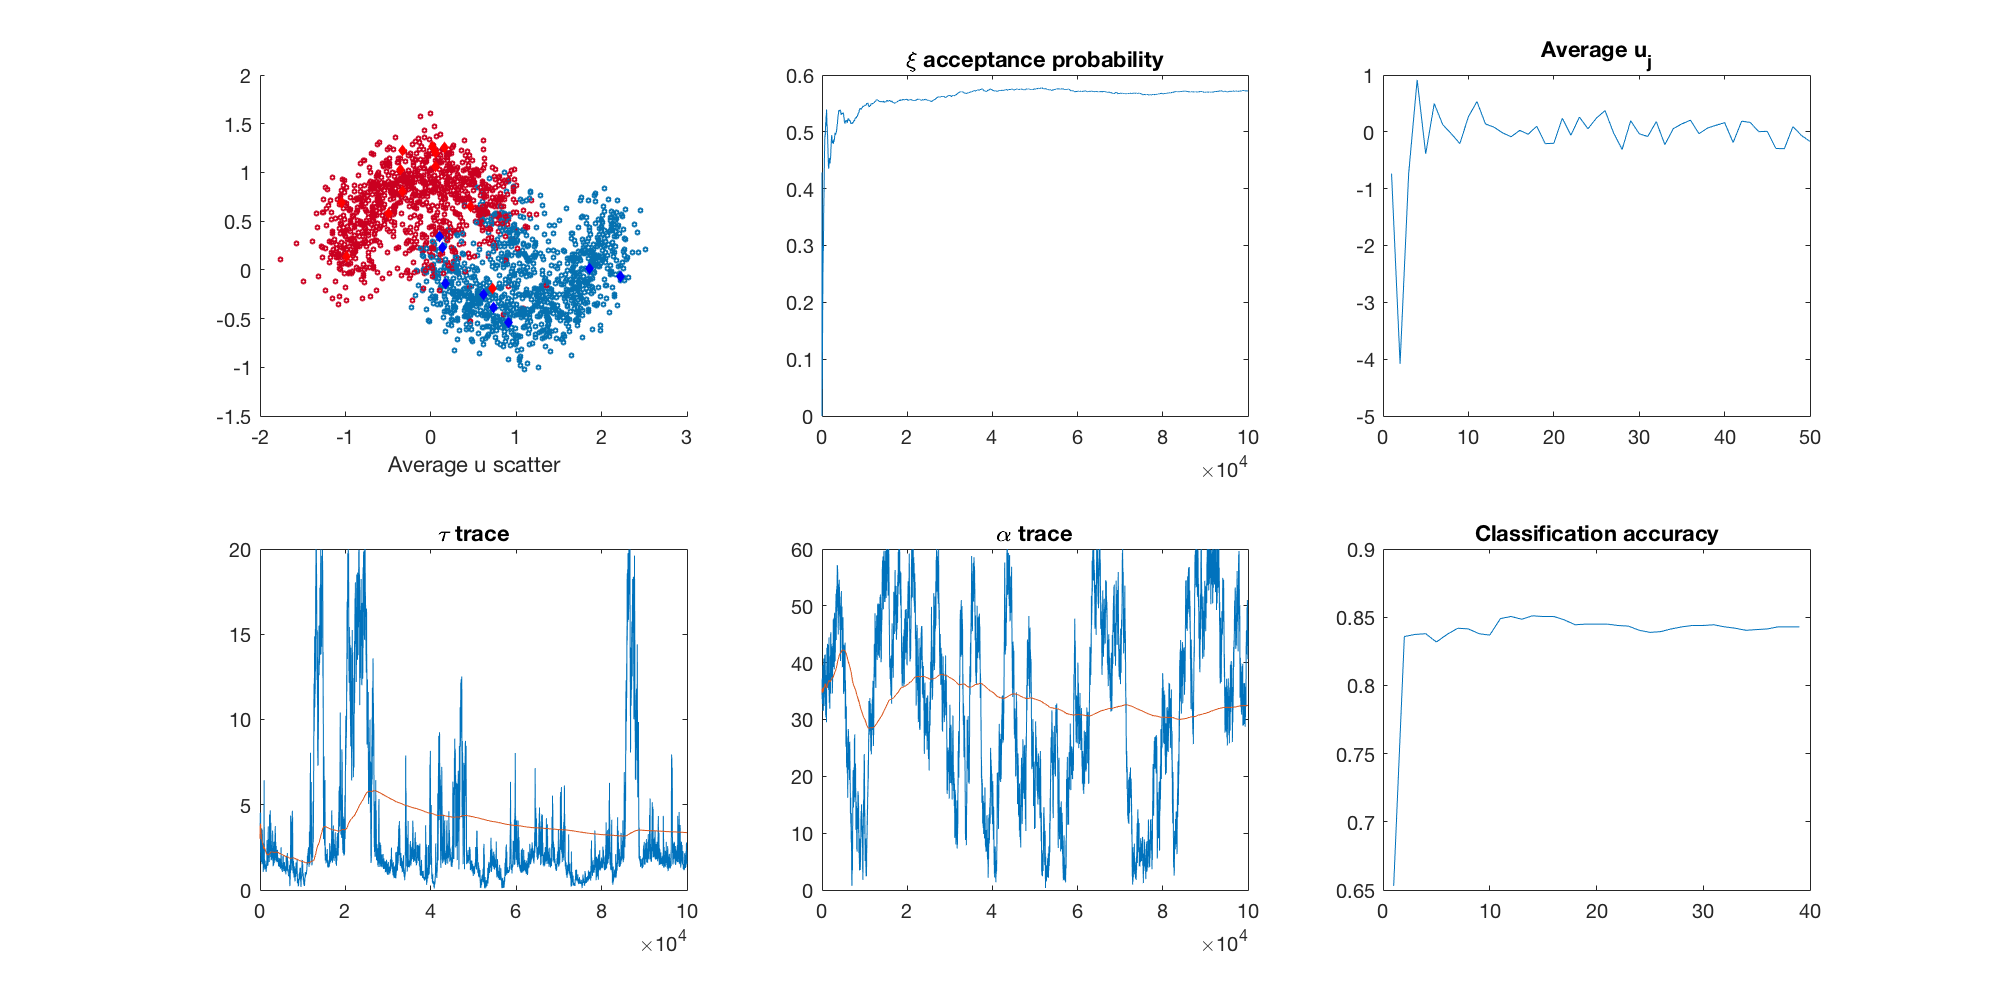
\includegraphics[width=\linewidth]{moons/learn_t_a/all.png}
        \end{figure}

        As shown in \cref{fig:model_c_two_moons}, this algorithm achieves around $85\%$ classification accuracy and the MCMC converges in both acceptance probability and classification accuracy after around $10000$ iterations.
    \subsection{Model (E)}
        If we choose the parameters of the prior on $v_j$ to be $\tau = 3, \alpha = 35, a=0.8$ and fix $M=50$ for model (E), we can obtain levels of accuracy and convergence rates similar to model (C). Note that this is ``cheating" in the sense that it uses the convergence of $\tau$ in model (C). The results are shown in \cref{fig:model_e_two_moons_t=3}.

        \begin{figure}[!htb]
            \caption{\label{fig:model_e_two_moons_t=3}Model (E) on two moons with $\tau=3,\alpha=35,a=0.8$. Figures from left to right, top to bottom: Final classification obtained, $\xi$ running acceptance probability, $v$ acceptance probability, final $v_j$ observation, final average of $u_j$, running classification accuracy (updated every 2500 trials).}
            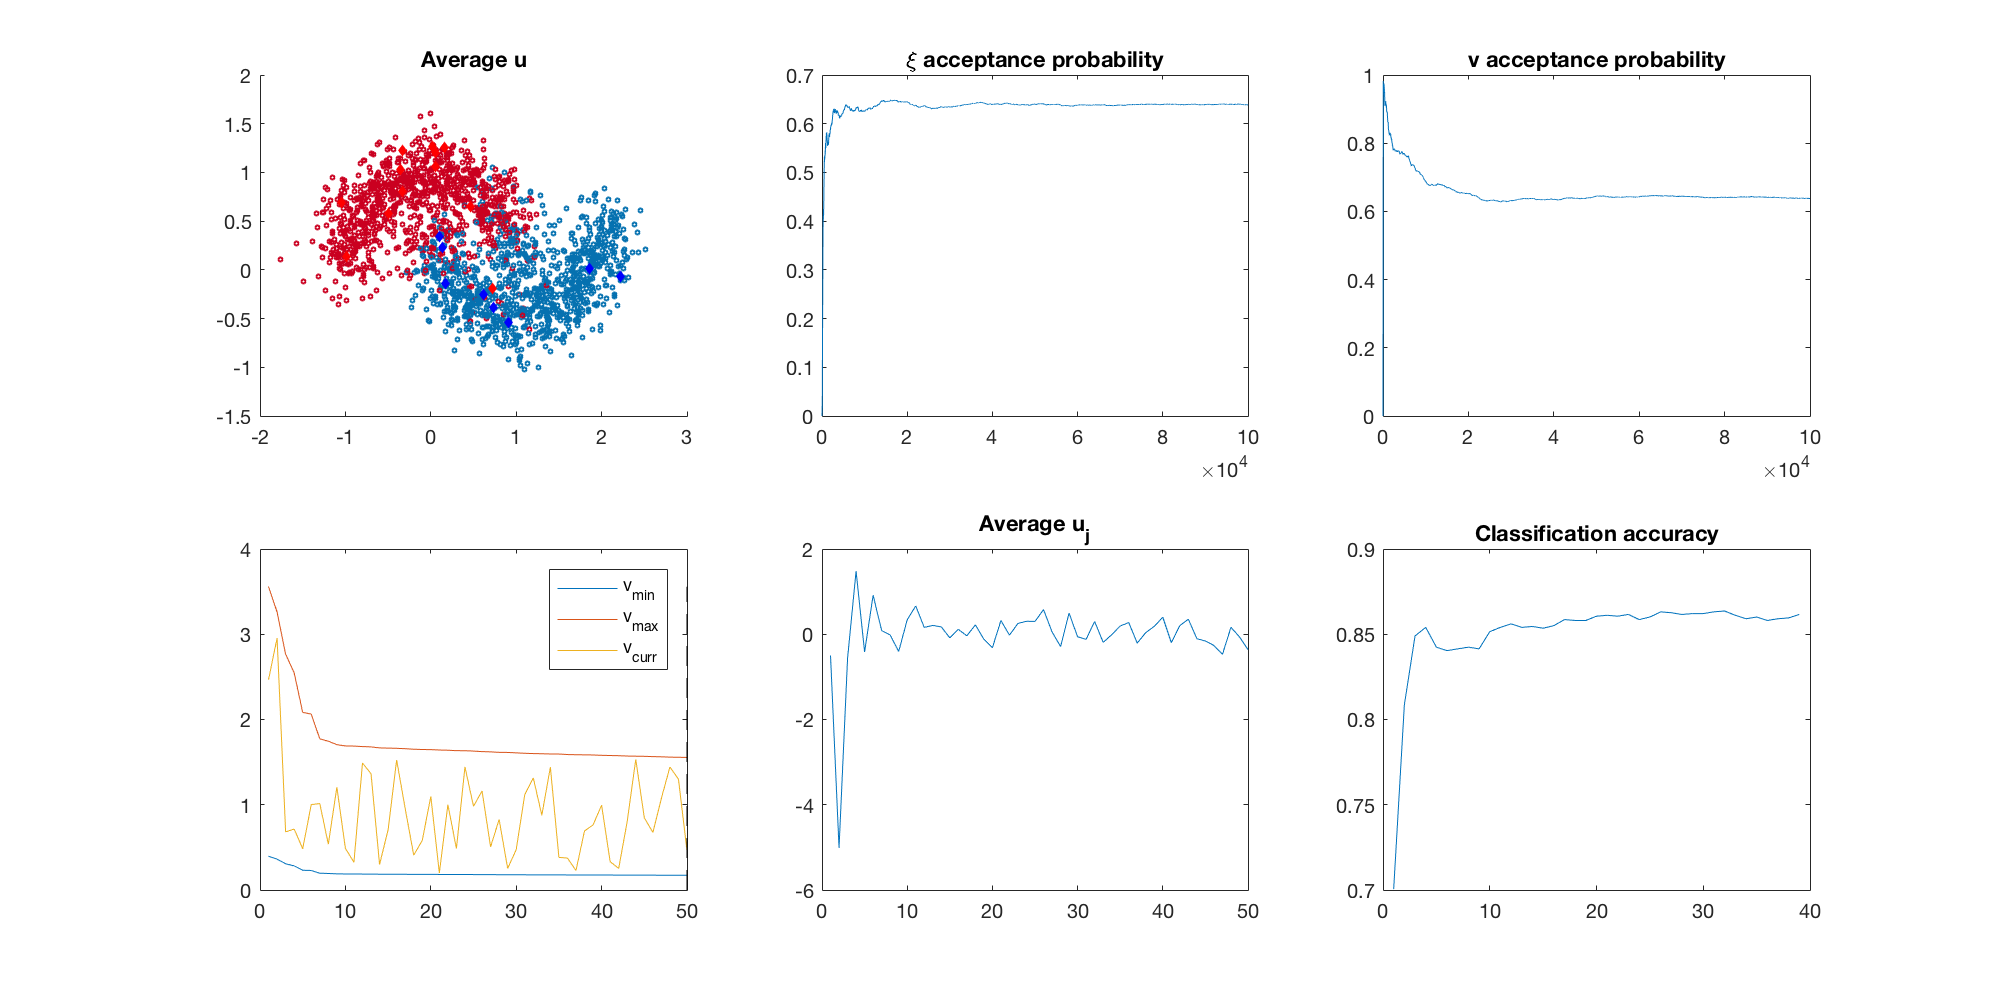
\includegraphics[width=\linewidth]{moons/learn_v/t=3.png}
        \end{figure}

        The same accuracy is not achieved when $\tau=5$ is chosen. See \cref{fig:model_e_two_moons_t=5}. Note that convergence of the classification accuracy appears much slower and the final accuracy is still lower than the previous two examples.

        \begin{figure}[!htb]
            \caption{\label{fig:model_e_two_moons_t=5}Model (E) on two moons with $\tau=5,\alpha=35,a=0.8$.}
            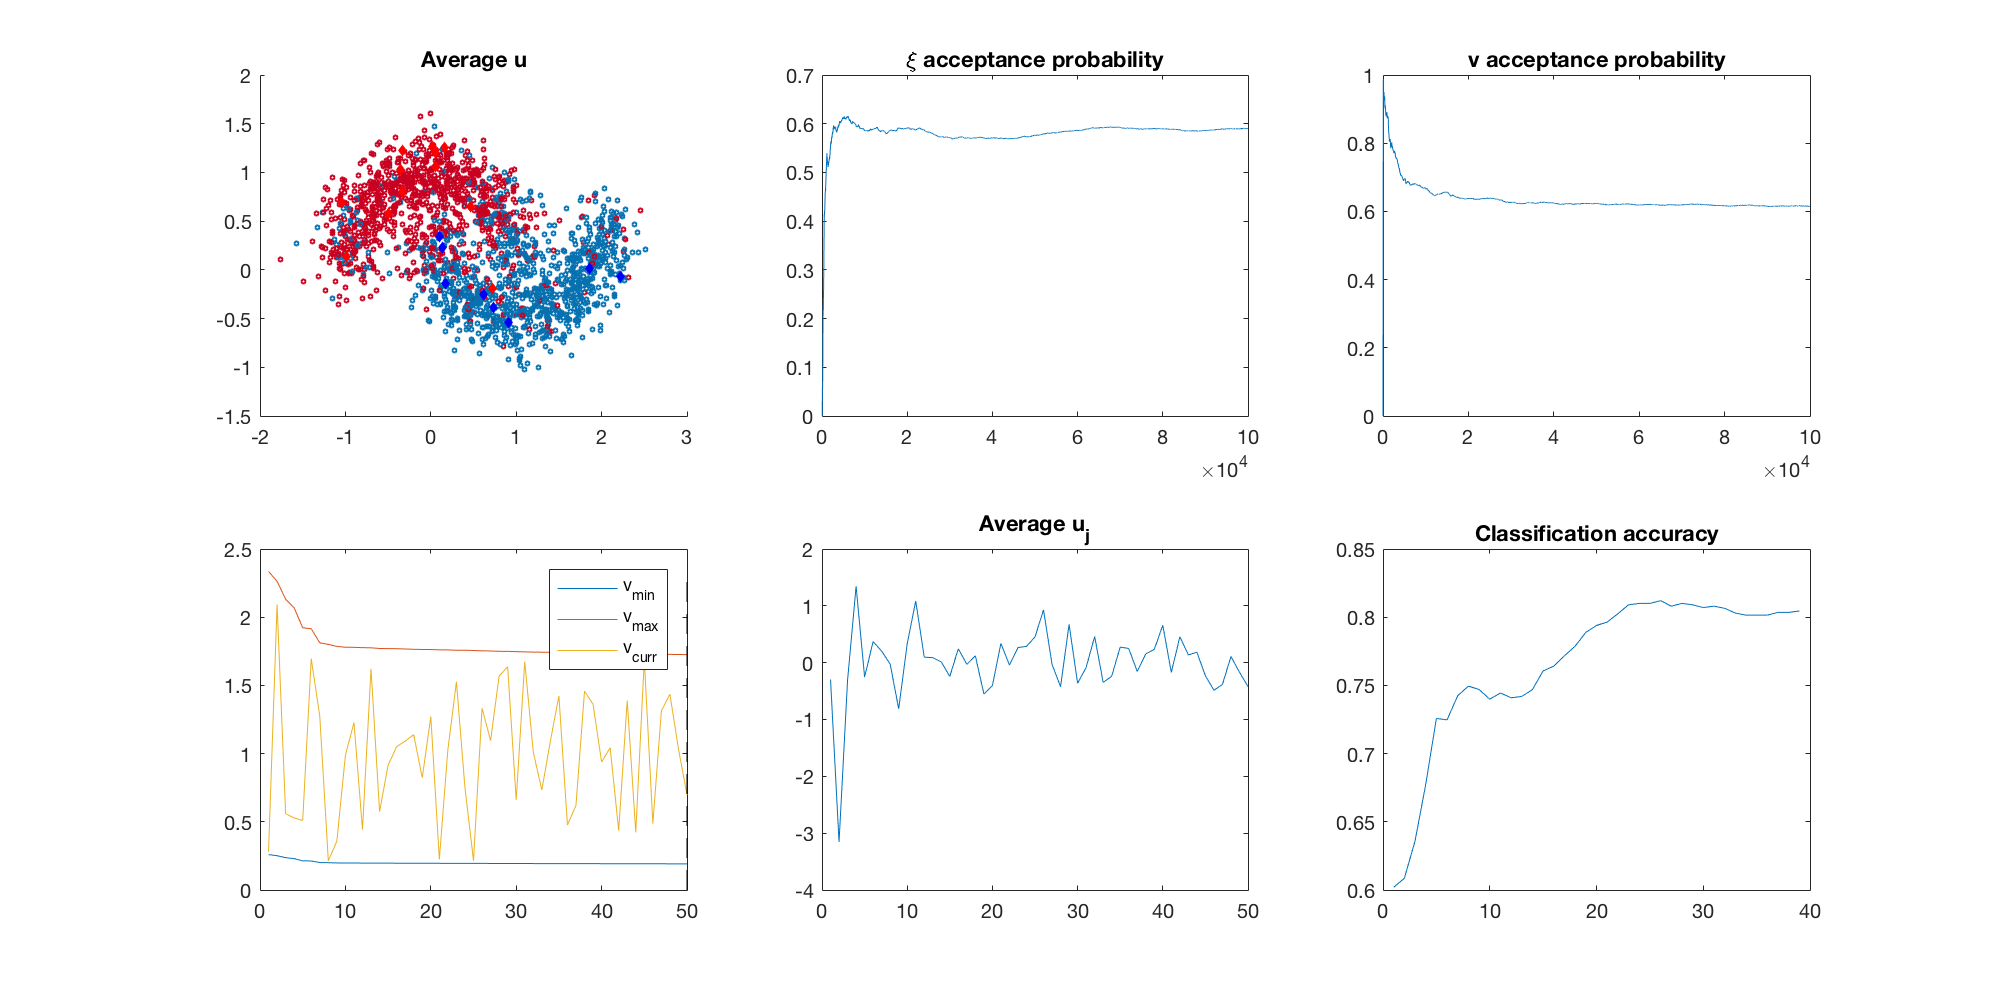
\includegraphics[width=\linewidth]{moons/learn_v/t=5.png}
        \end{figure}

        It seems that model (E) is very sensitive to the value of $\tau$ chosen for its prior. Initializing $\tau$ to be at the value suggested by model (C) achieves similar results in both classification accuracy and convergence rate, but choosing a somewhat poor value of $\tau$ leads to a noticeable drop in accuracy and convergence rate.

\section{MNIST}
    We compare these two algorithms on MNIST binary classification of $4$ and $9$. We set $\gamma = 0.0001$ for the label noise (this seems to improve accuracy for both models).
        \subsection{Model (C)}
            We fix $M=50$ and allow $\tau, \alpha$ to be learnt from uniform priors $[0.01, 20]$ and $[0.1, 60]$, respectively. The results are shown in \cref{fig:model_c_mnist}. $\tau$ is initialized at $20$ but finds a small value at around step $20000$ and stays around there. Note that this corresponds with the sharp increase in classification accuracy after this value of $\tau$ was found. The mean and median of $\tau$ after it seems to converge is around $0.7$. The accuracy is around $96\%$.
        \begin{figure}[!htb]
            \caption{\label{fig:model_c_mnist}Model (C) on MNIST49. Figures from top to bottom, left to right: Final classification obtained, $\xi$ running acceptance probability, final average of $u_j$, $\tau$ trace, $\alpha$ trace, running classification accuracy (updated every 2500 trials).}
            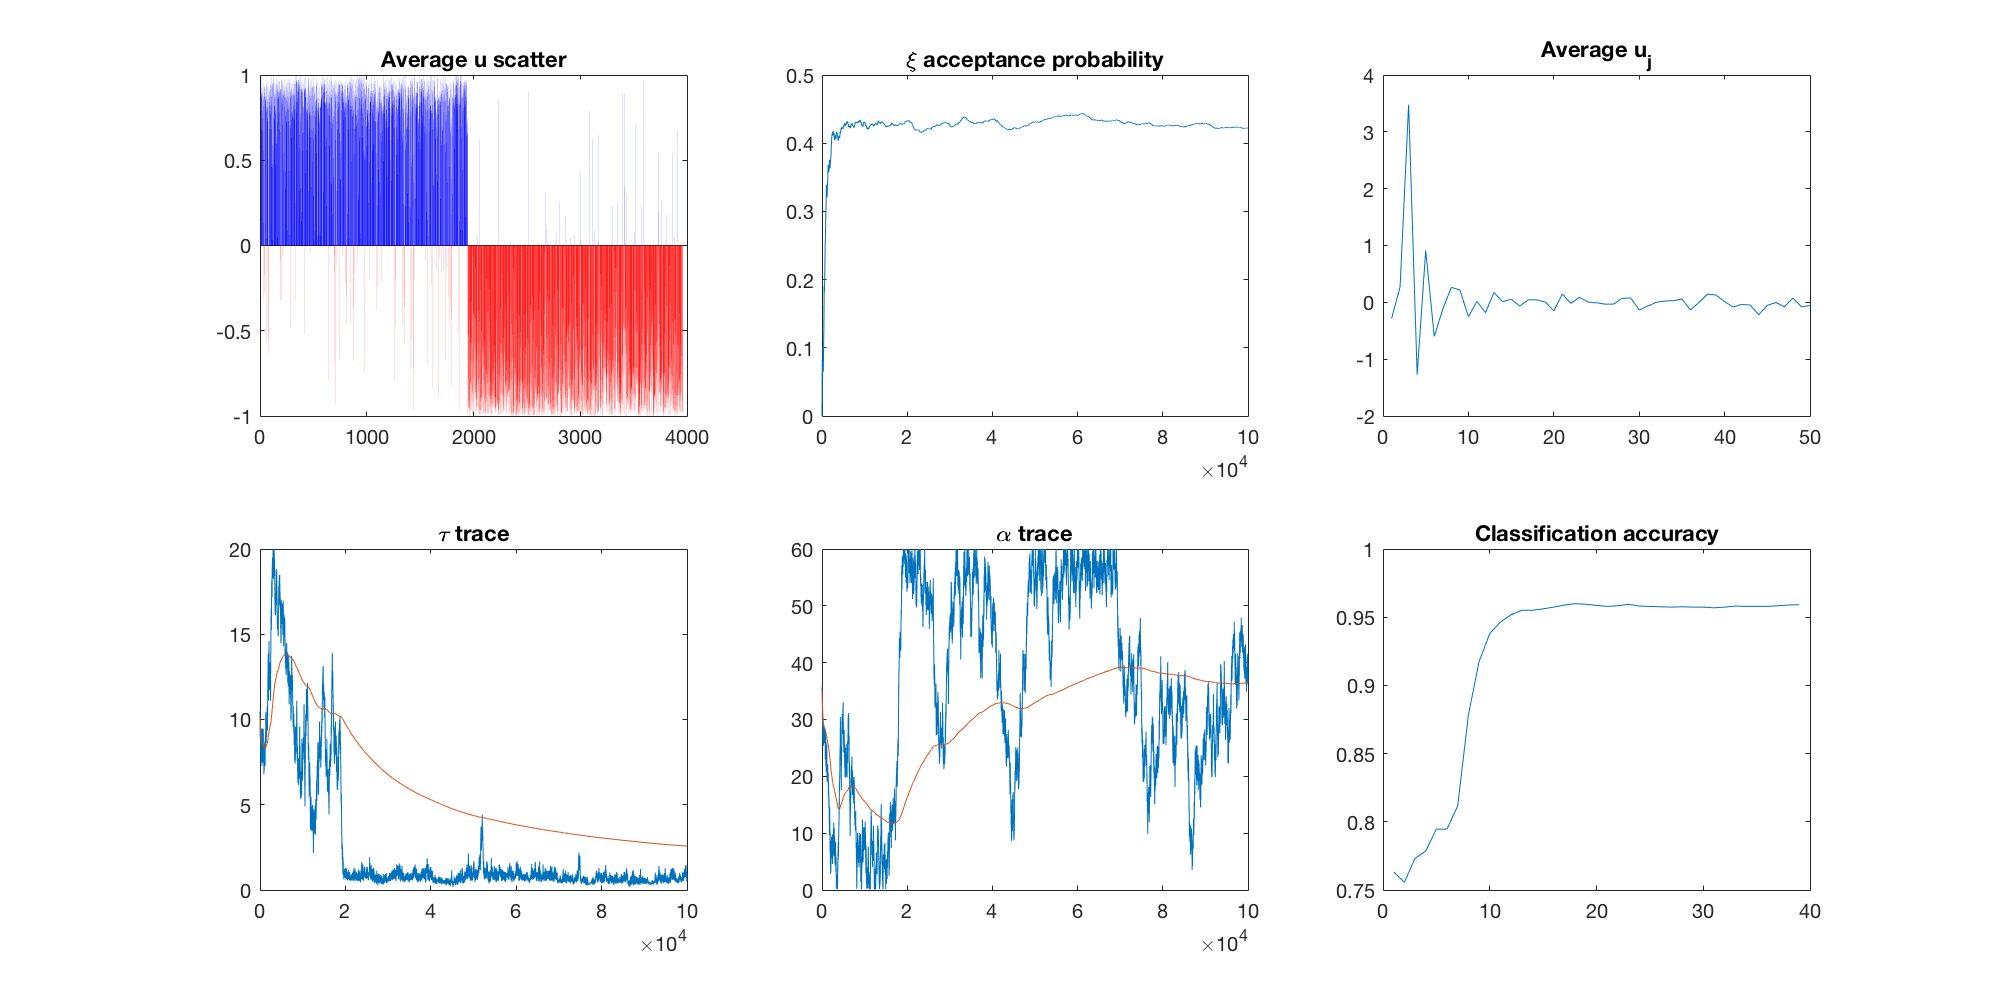
\includegraphics[width=\linewidth]{mnist/learn_t_a/all.png}
        \end{figure}
        \subsection{Model (E)}
            Fix $M=50$ again. 
            With $\tau = 0.7$ (which is ``cheating" by using the $\tau$ learnt from model (C)), we obtain \cref{fig:model_e_mnist_t=0.7}. Note the similar final accuracy of around $96\%$, with faster convergence to that accuracy since we cheated with the initialization.
            \begin{figure}[!htb]
            \caption{\label{fig:model_e_mnist_t=0.7}Model (E) on two moons with $\tau=0.7,\alpha=35,a=0.8$. Figures from left to right, top to bottom: Final classification obtained, $\xi$ running acceptance probability, $v$ acceptance probability, final $v_j$ observation, final average of $u_j$, running classification accuracy (updated every 2500 trials).}
            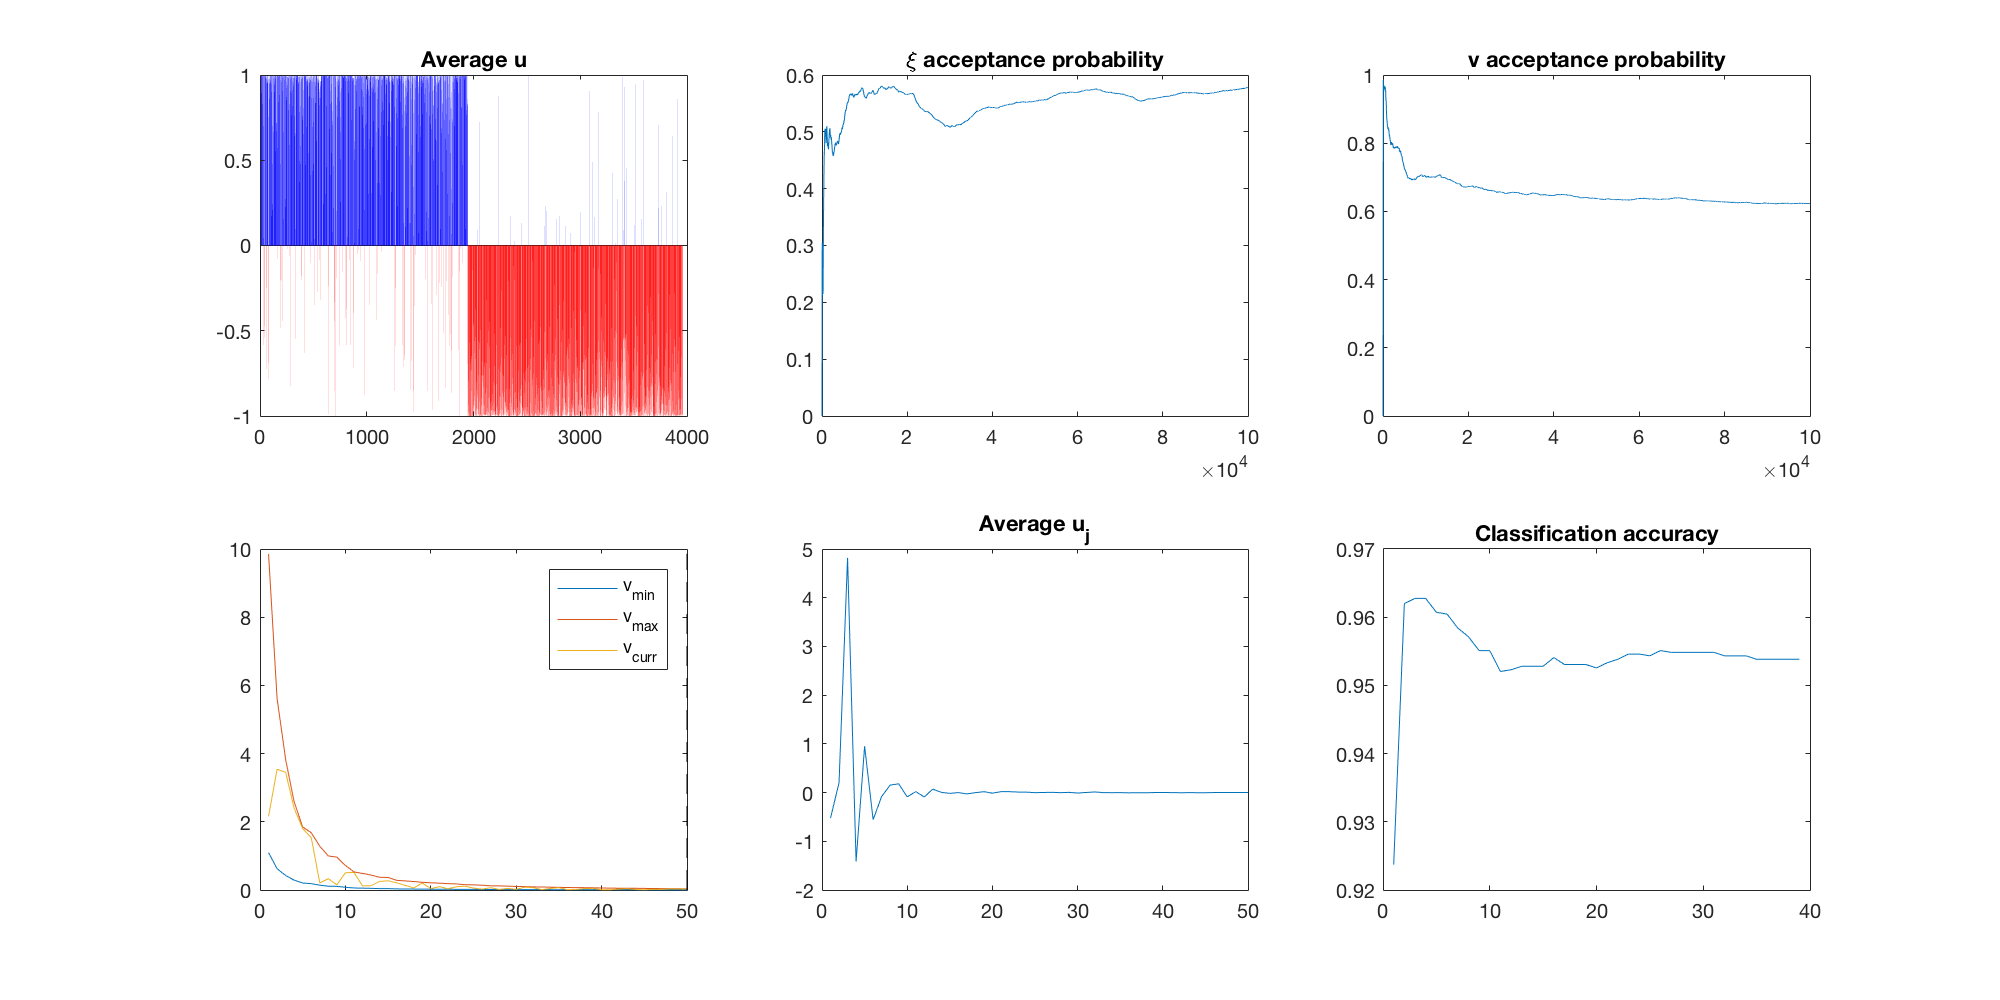
\includegraphics[width=\linewidth]{mnist/learn_v/t=0_7.png}
            \end{figure}

            With $\tau = 0.3$, we obtain \cref{fig:model_e_mnist_t=0.3}. Note the slow convergence compared to $\tau=0.7$. In fact, it appears that the accuracy is still climbing even at 100000 iterations.
            \begin{figure}[!htb]
            \caption{\label{fig:model_e_mnist_t=0.3}Model (E) on two moons with $\tau=0.3,\alpha=35,a=0.8$.}
            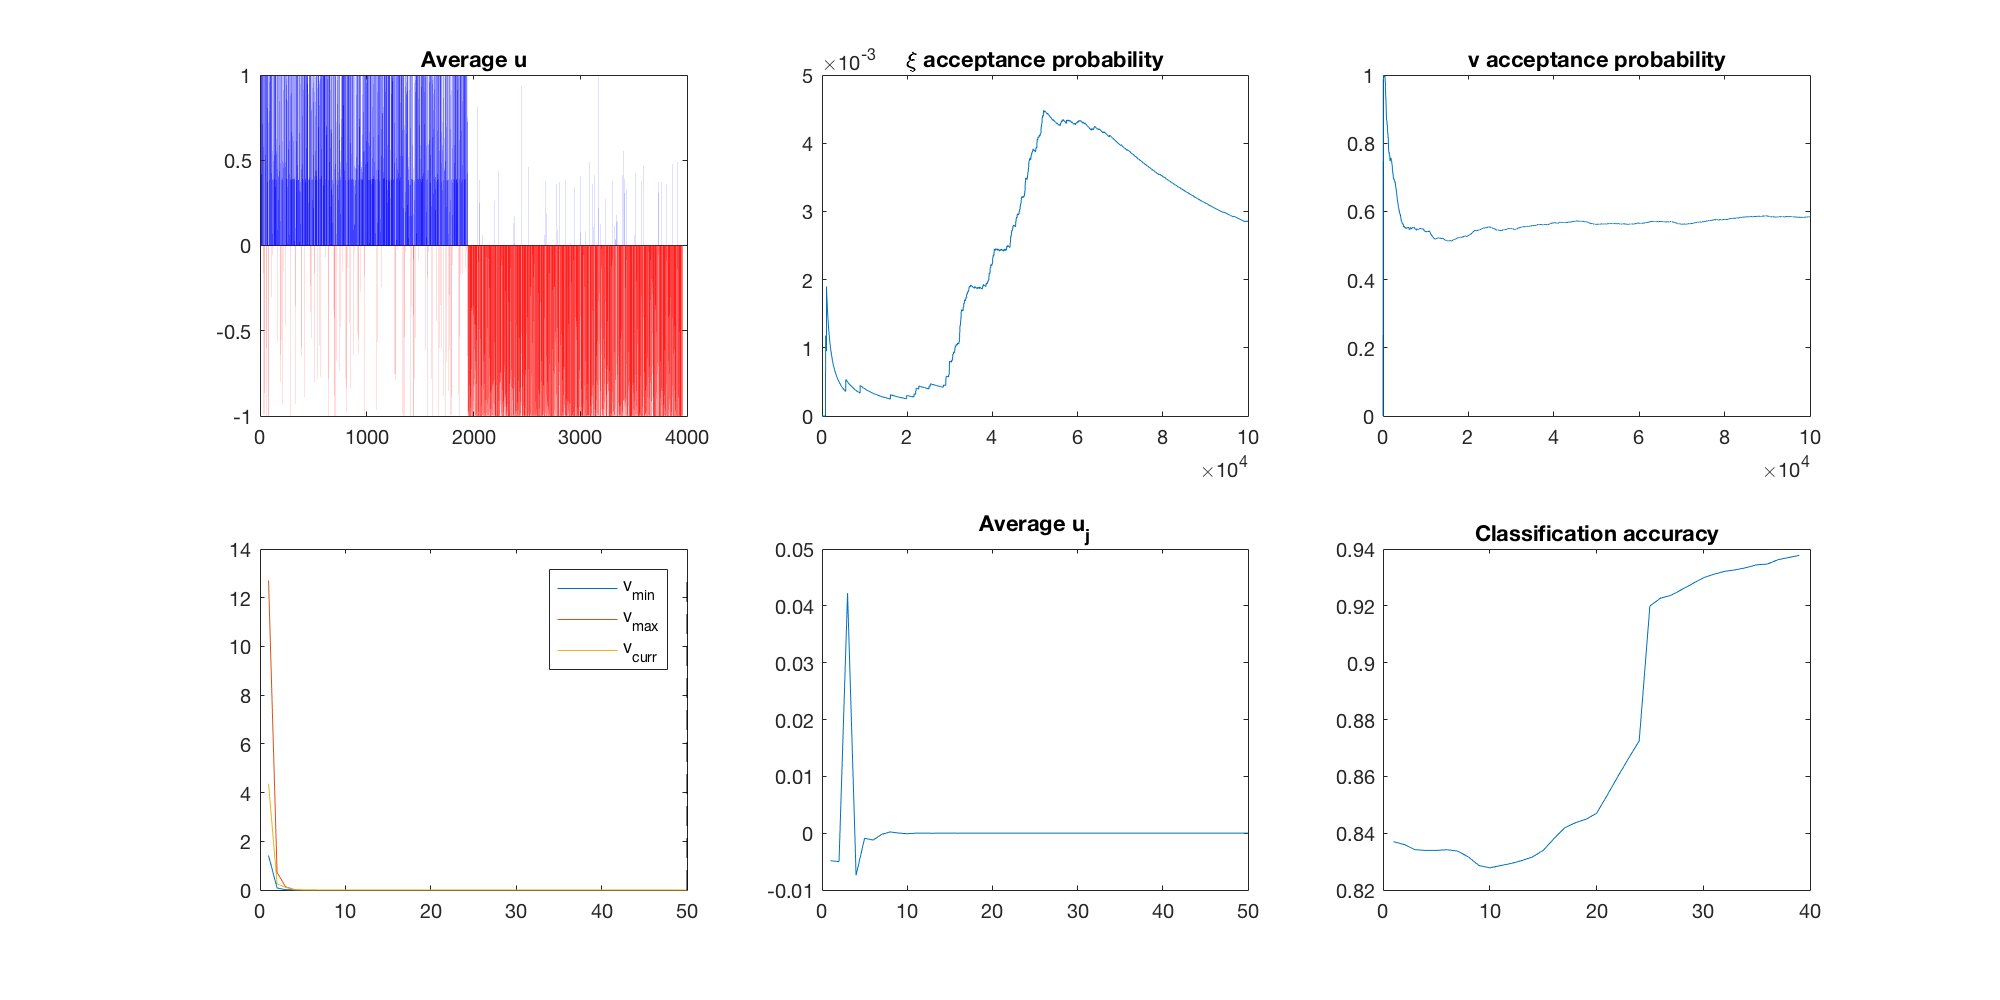
\includegraphics[width=\linewidth]{mnist/learn_v/t=0_3.png}
            \end{figure}

            With $\tau = 5$, we obtain \cref{fig:model_e_mnist_t=5}. Note the overall lower final accuracy of around $90\%$.
            \begin{figure}[!htb]
            \caption{\label{fig:model_e_mnist_t=5}Model (E) on two moons with $\tau=5,\alpha=35,a=0.8$.}
            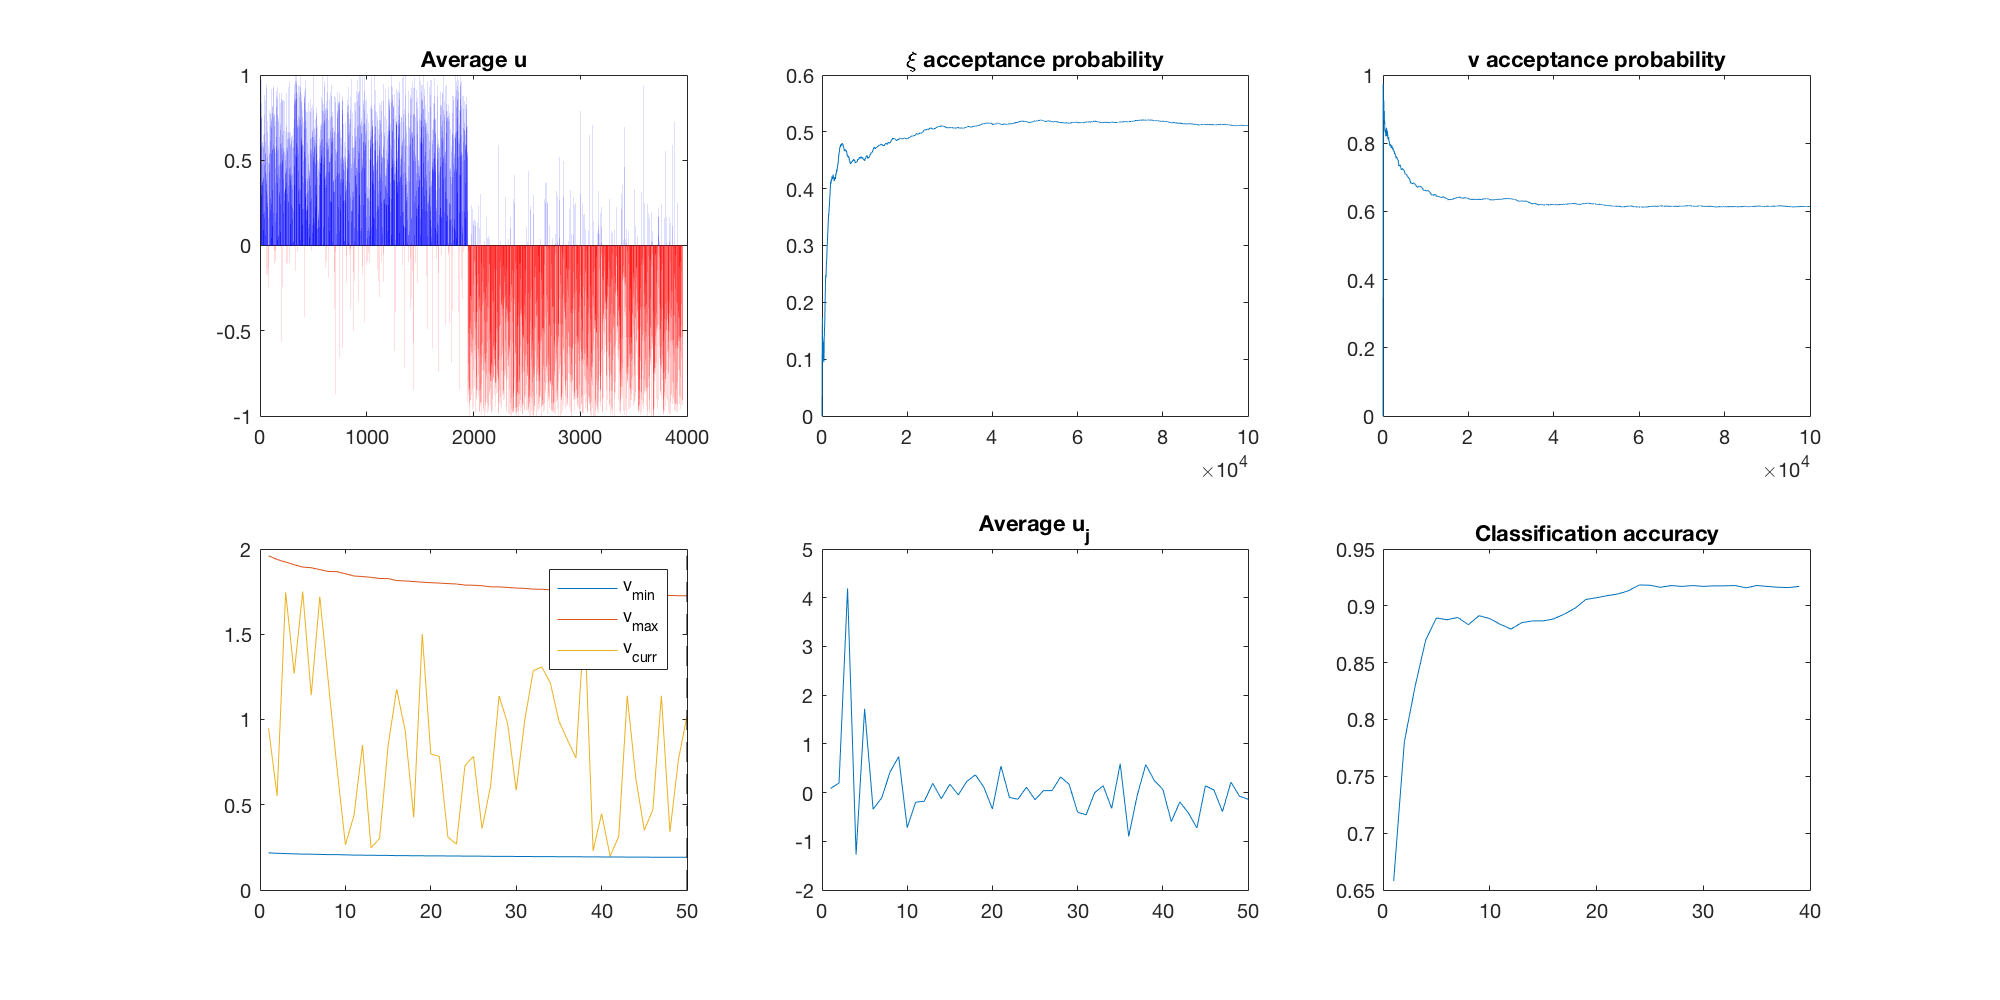
\includegraphics[width=\linewidth]{mnist/learn_v/t=5.png}
            \end{figure}

\section{Observations on $\tau, \alpha$}
    This section attempts to summarize the discussions on the effects of $\tau$ and $\alpha$.

    With small fixed values of $\alpha$, such as $\alpha=1$, the variance of the Gaussian prior on $u_j$ decreases at a slower rate with increasing values of $j$. This means that the algorithm is more able to draw samples that use eigenvectors with a large range of indices. If the problem can be solved with a small number of eigenvectors, we expect $\alpha$ to be larger.

    The smallest eigenvectors of the graph Laplacian should behave as indicators of the clusters and have eigenvalues close to zero. This means $\lambda + \tau^2$ will appear to be close to $\tau^2$ for these eigenvectors. $\tau$ should be large enough so that the eigenvectors needed have similar values of $\lambda + \tau^2$, but must be small enough so that the unnecessary eigenvectors do not also appear to have the same value of $\lambda + \tau^2$.

\bibliographystyle{siamplain}
\bibliography{references}
\end{document}